\documentclass[PhD-Yoann-Dupont.tex]{subfiles}
\begin{document}

Les programmes implémentant les CRF génèrent leurs features d'une des deux façons suivantes. Dans la première, seules les features réellement observées sur l'ensemble d'apprentissage sont générées. La seconde génère l'ensemble des features qu'il est possible de générer étant donné un jeu d'observations, autrement dit, toutes les possibles associations observation/étiquette sont générées dans le modèle. Le premier cas a l'avantage de générer un nombre réduit de traits et donne des modèles rapides et légers, mais qui généralisent assez mal. Le second cas permet d'avoir une meilleure généralisation et des calculs mathématiques plus simples et optimisables, au prix d'une plus grande consommation mémoire. Dans le cadre de l'apprentissage en utilisant un schéma d'annotation BIO ou BILOU, nous pouvons arguer pour un entre-deux, permettant d'avoir un nombre réduit de traits tout en gardant la même expressivité qu'un modèle complet. En effet, nombre de transitions dans un schéma BIO ou BILOU sont inconsistantes dans le monde réel. Dans le schéma BIO, si nous avons deux classes A et B, la transition $I-A\ \rightarrow I-B$ est inconsistante, elle n'a aucun pouvoir d'expression et il est tout à fait raisonnable de ne pas générer les features bigrammes correspondant à cette transition. L'idée est ici est d'utiliser le schéma d'annotation pour élaguer noeuds/transition dans forward-backward et/ou Viterbi. Dans la suite, nous nous concentrerons sur le schéma BILOU, pour lequel les résultats sont plus intéressants. Supposons que nous avons deux classes de sortie : \emph{Person} et \emph{Location}. Les figures \ref{fig:BILOU-transition-from-BI} et \ref{fig:BILOU-transition-from-LUO} montrent les transitions consistantes dans un schéma BILOU. Un comparatif du nombre de transitions générées par le schéma BILOU par rapport au schéma BIO est donné dans la figure \ref{fig:bio-to-bilou-consumption}.

    \begin{figure}[ht!]
    \centering
        \begin{tikzpicture}[thick,
          every node/.style={draw=none,circle},
          fsnode/.style={draw=none},
          ssnode/.style={draw=none},
          %every fit/.style={ellipse,draw,inner sep=-2pt,text width=2cm},
          %->,shorten >= 3pt,shorten <= 3pt
        ]

        % the vertices of left side
        \begin{scope}[start chain=going below,node distance=7mm]
        \node[fsnode,on chain] (left-b-person) [label=left: B-Person] {};
        \node[fsnode,on chain] (left-i-person) [label=left: I-Person] {};
        \node[fsnode,on chain] (left-l-person) [label=left: L-Person] {};
        \node[fsnode,on chain] (left-u-person) [label=left: U-Person] {};
        \node[fsnode,on chain] (left-b-location) [label=left: B-Location] {};
        \node[fsnode,on chain] (left-i-location) [label=left: I-Location] {};
        \node[fsnode,on chain] (left-l-location) [label=left: L-Location] {};
        \node[fsnode,on chain] (left-u-location) [label=left: U-Location] {};
        \node[fsnode,on chain] (left-o) [label=left: O] {};
        \end{scope}

        % the vertices of right side
        \begin{scope}[xshift=4cm,start chain=going below,node distance=7mm]
        \node[fsnode,on chain] (right-b-person) [label=right: B-Person] {};
        \node[fsnode,on chain] (right-i-person) [label=right: I-Person] {};
        \node[fsnode,on chain] (right-l-person) [label=right: L-Person] {};
        \node[fsnode,on chain] (right-u-person) [label=right: U-Person] {};
        \node[fsnode,on chain] (right-b-location) [label=right: B-Location] {};
        \node[fsnode,on chain] (right-i-location) [label=right: I-Location] {};
        \node[fsnode,on chain] (right-l-location) [label=right: L-Location] {};
        \node[fsnode,on chain] (right-u-location) [label=right: U-Location] {};
        \node[fsnode,on chain] (right-o) [label=right: O] {};
        \end{scope}

        % the set U
        \node [fit=(left-b-person) (left-o),label=above:$t-1$] {};
        % the set V
        \node [fit=(right-b-person) (right-o),label=above:$t$] {};

        % the edges
        \draw[->] (left-b-person) -> (right-i-person);
        \draw[->] (left-b-person) -> (right-l-person);
        %\draw (left-) -- (right-);
        \end{tikzpicture}
    \caption{Les transitions possibles depuis une étiquette $B-*$. Ces transitions sont valables pour les étiquettes $I-*$ également.}
    \label{fig:BILOU-transition-from-BI}
    \end{figure}

    \begin{figure}[ht!]
        \centering
        \begin{tikzpicture}[thick,
          every node/.style={draw=none,circle},
          fsnode/.style={draw=none},
          ssnode/.style={draw=none},
          %every fit/.style={ellipse,draw,inner sep=-2pt,text width=2cm},
          %->,shorten >= 3pt,shorten <= 3pt
        ]

        % the vertices of left side
        \begin{scope}[start chain=going below,node distance=7mm]
        \node[fsnode,on chain] (left-b-person) [label=left: B-Person] {};
        \node[fsnode,on chain] (left-i-person) [label=left: I-Person] {};
        \node[fsnode,on chain] (left-l-person) [label=left: L-Person] {};
        \node[fsnode,on chain] (left-u-person) [label=left: U-Person] {};
        \node[fsnode,on chain] (left-b-location) [label=left: B-Location] {};
        \node[fsnode,on chain] (left-i-location) [label=left: I-Location] {};
        \node[fsnode,on chain] (left-l-location) [label=left: L-Location] {};
        \node[fsnode,on chain] (left-u-location) [label=left: U-Location] {};
        \node[fsnode,on chain] (left-o) [label=left: O] {};
        \end{scope}

        % the vertices of right side
        \begin{scope}[xshift=4cm,start chain=going below,node distance=7mm]
        \node[fsnode,on chain] (right-b-person) [label=right: B-Person] {};
        \node[fsnode,on chain] (right-i-person) [label=right: I-Person] {};
        \node[fsnode,on chain] (right-l-person) [label=right: L-Person] {};
        \node[fsnode,on chain] (right-u-person) [label=right: U-Person] {};
        \node[fsnode,on chain] (right-b-location) [label=right: B-Location] {};
        \node[fsnode,on chain] (right-i-location) [label=right: I-Location] {};
        \node[fsnode,on chain] (right-l-location) [label=right: L-Location] {};
        \node[fsnode,on chain] (right-u-location) [label=right: U-Location] {};
        \node[fsnode,on chain] (right-o) [label=right: O] {};
        \end{scope}

        % the set U
        \node [fit=(left-b-person) (left-o),label=above:$t-1$] {};
        % the set V
        \node [fit=(right-b-person) (right-o),label=above:$t$] {};

        % the edges
        \draw[->] (left-l-person) -> (right-b-person);
        \draw[->] (left-l-person) -> (right-u-person);
        \draw[->] (left-l-person) -> (right-b-location);
        \draw[->] (left-l-person) -> (right-u-location);
        \draw[->] (left-l-person) -> (right-o);
        %\draw (left-) -- (right-);
        \end{tikzpicture}
    \caption{Les transitions possibles depuis une étiquette $L-*$. Ces transitions sont valables pour les étiquettes $U-*$ et $O$ également.}
    \label{fig:BILOU-transition-from-LUO}
    \end{figure}
    
    \begin{figure}[ht!]
    \centering
        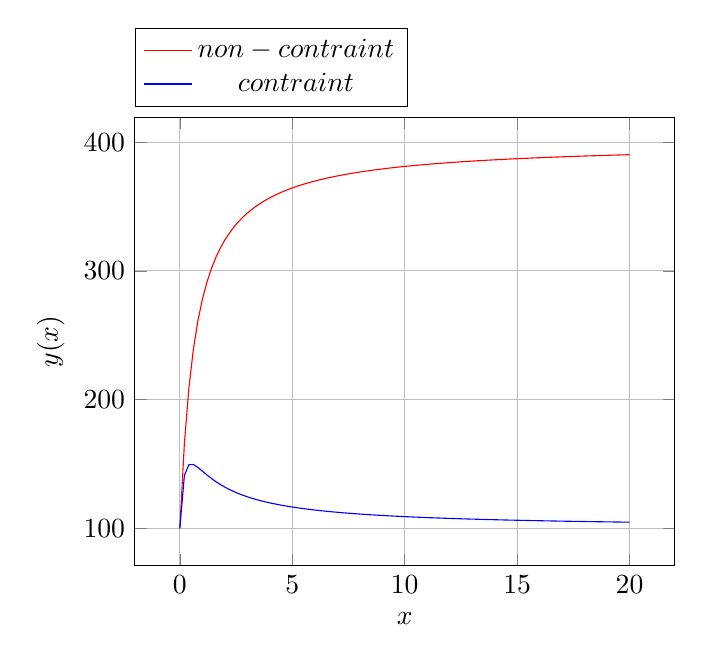
\begin{tikzpicture}
        \begin{axis}[domain=0:20, samples=100,grid=major,restrict expr to domain=0:100,restrict y to domain=0:400,xlabel=$x$,ylabel=$y(x)$, legend style={at={(0.0,1.2)},anchor=north west}]
        \addplot [color=red]  {100*(((4*x+1)*(4*x+1))/((2*x+1)*(2*x+1)))};
        \addplot [color=blue] {100*(((4*x)+((2*x+1)*(2*x+1)))/((2*x+1)*(2*x+1)))};
        \legend{$non-contraint$,$contraint$}
        \end{axis}
        \end{tikzpicture}
    \caption{augmentation du nombre de transitions en passant d'un schéma BIO au schéma BILOU en fonction du nombre de classes de sorties. En rouge, le nombre de transitions sans contrainte d'intégrité. En bleu, le nombre de transition respectant les contraintes d'intégrité.}
    \label{fig:bio-to-bilou-consumption}
    \end{figure}

\end{document}